\section{Experimentos y análisis}

A continuación analizaremos los resultados de algunos experimentos realizados con la herramienta desarrollada.
\\\\
Para los experimentos elegimos tres universidades de continentes diferentes para analizar las rutas tomadas por los paquetes hacia las mismas. Las universidades que elegimos son:
\begin{itemize}
\item Universidad de Sydney, Australia: sydney.edu.au
\item Universidad de Ciencia y Tecnología de Trondheim, Noruega: ntnu.edu
\item Universidad de Shanghai, China: shu.edu.cn
\end{itemize}
\subsection{Universidad de Australia}
Para analizar los resultados obtenidos con la Universidad de Sydney, Australia (sydney.edu.au) primero veremos un gráfico que muestra los valores de los RTT obtenidos para cada salto (TTL).

\FloatBarrier

\begin{figure}[ht!]
  \centering
   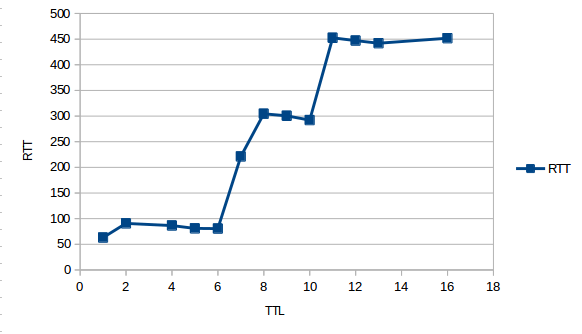
\includegraphics[width=0.7\textwidth]{imagenes/AUS.png}
\end{figure}

\FloatBarrier

Se puede observar lo que parecen ser dos grandes saltos, uno entre el TTL 6 y 7, y otro entre el TTL 10 y 11. Estos dos saltos parecerían candidatos a ser enlaces intercontinentales. 
\\
Otro detalle que podemos observar es que hay valores de RTT que disminuyen con respecto al anterior, cuando sería de esperar que el RTT aumente en cada salto.
Por último, se puede ver que para algunos saltos, no se ven valores de RTT. Esto se debe a que para algunos valores de TTL, el nodo no retornó respuesta. Posiblemente por tener deshabilitado el protocolo ICMP.
\\\\
A continuación se muestran los resultados obtenidos por nuestra herramienta \texttt{traceroute} y realizaremos un análisis más detallado.     

\begin{center}
    \begin{tabular}{| l | l | l | l | l | }
    \hline
    Saltos & IP                       & RTT   & DRTT     & País       \\ \hline
    1         &  192.168.1.1      & 67.0   &  67.0       & Local          \\ \hline
    2         &  201.254.128.1  & 77.23 & 10.23      & Argentina   \\ \hline
    3   	    & *****                   &           &               &                    \\ \hline
    4   	    & 200.51.208.90   & 86.1   & 8.87       & Argentina    \\ \hline
    5   	    & 200.51.240.181 & 89.83 & 3.73       & Argentina    \\ \hline
    6   	    & 213.140.39.118 & 84.63 & -5.2        & Argentina \\ \hline
    7   	    & 176.52.255.27   & 221.7   & 137.07 &  United States  \\ \hline
    8   	    & 213.140.36.70   & 303.3   & 81.6     & United States \\ \hline
    9   	    & 213.140.52.229 & 284.67 & -18.63  &  United States  \\ \hline
  10   	    & 208.185.52.74   & 300.2   & 15.53   & United States \\ \hline
  11   	    & 202.158.194.176 & 443.4 & 143.2   & Australia  \\ \hline
  12   	    & 113.197.15.146  & 446.6  & 3.2       & Australia \\ \hline
  13   	    & 138.44.5.47        & 443.23 & -3.37   & Australia \\ \hline
  14   	    & *****                    &              &           & \\ \hline
  15   	    & *****                    &              &           &\\ \hline
  16   	    & 129.78.5.8          & 447.28  &  4.04  & Australia \\ \hline

  \end{tabular}
\end{center}

Podemos notar que para los saltos 3, 14 y 15 no se obtuvo respuesta. Esta posiblemente sea una anomalía de \texttt{traceroute} conocida como \emph{Missing Hops}. Por lo general ocurre cuando un router está protegido por un firewall o configurado para no generar paquetes \emph{ICMP Time Exceeded}.   
\\
También podemos observar algunos valores negativos, en los saltos 6, 9 y 13. Esto puede ser porque se presenta un tipo de anomalía llamada \emph{False Round-Trip Times}. Este caso suele darse cuando los tiempos de ida y vuelta de un paquete reportados por \texttt{traceroute} son erróneos. Por lo general puede haber dos razones que generan este comportamiento. Rutas de paquetes asimétricas o enrutamiento MPLS. 
\\
Cuando los respectivos caminos hacia y desde el destino son asimétricos, es decir, que los paquetes se encaminan por caminos diferentes, los tiempos de ida y vuelta pueden no reflejar el RTT real.
\\
Un resultado similar se produce en los enlaces MPLS, donde el paquete tiene que viajar hasta el final de la ruta MPLS, antes de que la respuesta se devuelva al origen. Dado que los routers que manejan exclusivamente MPLS solamente conocen el siguiente salto, no pueden enviar \emph{ICMP Time Exceeded} directamente. En su lugar, tienen que utilizar la ruta por donde el paquete original habría ido. El resultado de esto es, que todos los paquetes viajan hasta el último router MPLS. Por lo tanto, para \texttt{traceroute}, los RTT de los saltos en el camino MPLS reflejan aproximadamente el RTT del último router MPLS.
\\\\
Ahora intentaremos inferir cuáles saltos son enlaces intercontinentales mediante la técnica de estimación de John M. Cimbala.
El resultado obtenido por nuestra herramienta fue que los siguientes saltos corresponden a enlaces intercontinentales.

\begin{center}
    \begin{tabular}{| l | l | l | l | l | }
    \hline
    Desde                & Hasta                  & DRTT   & País Desde      & País Hasta \\ \hline
    208.185.52.74   & 202.158.194.176 & 143.2   &  United States  & Australia      \\ \hline
    213.140.39.118 & 176.52.255.27     & 137.07 &  Argentina        & United States \\ \hline
    176.52.255.27   & 213.140.36.70     & 81.6     &United States    & United States \\ \hline
  \end{tabular}
\end{center}

Como podemos observar, los dos primeros outliers sugeridos por la herramienta parecerían efectivamente ser enlaces intercontinentales.
\\
Para verificar esta hipótesis nos apoyamos en la información provista por sitios de geolocalización de direcciones IP y pudimos comprobar lo siguiente.
\\
El primer salto corresponde a un enlace entre un router de Argentina con uno de Estados Unidos. El segundo, es desde un router de Estados Unidos a uno de Australia.
\\
La herramienta, sugirió un tercer outlier, pero según el análisis de geolocalización que pudimos realizar parecería no representar un enlace intercontinental. Si bien las herramientas de geolocalización ubica al router con dirección IP 176.52.255.27 en España. Pudimos observar que el nombre de este host es hu0-11-0-0-grtmiabr5, donde el texto “mia” corresponde a la abreviación de Miami. Por lo tanto deducimos que corresponde a un router ubicado en Estados Unidos con una dirección IP española asignada. 
\\\\
A continuación veremos en un mapa las direcciones IP de los diferentes saltos, ubicadas según el análisis realizado.

\FloatBarrier

\begin{figure}[ht!]
  \centering
   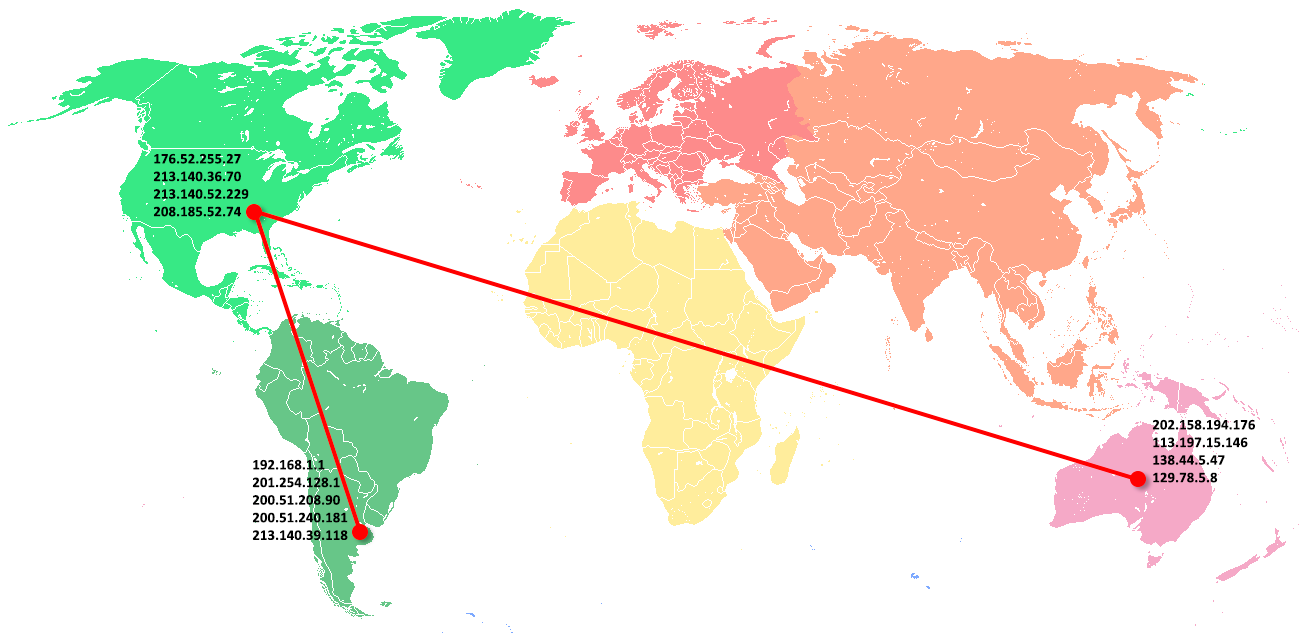
\includegraphics[width=1.0\textwidth]{imagenes/mapaAUS.png}
\end{figure}

\FloatBarrier

Si bien en el mapa se muestran los enlaces como líneas rectas, para el caso del enlace entre Estados Unidos y Australia, lo más probable es que este en realidad atraviese el océano Atlántico.

\subsection{Universidad de China}
En segundo lugar realizamos el análisis de los datos para la Universidad de Shanghai, China (shu.edu.cn). 
A continuación veremos el gráfico que muestra los valores de los RTT en cada salto (TTL).

\FloatBarrier

\begin{figure}[ht!]
  \centering
   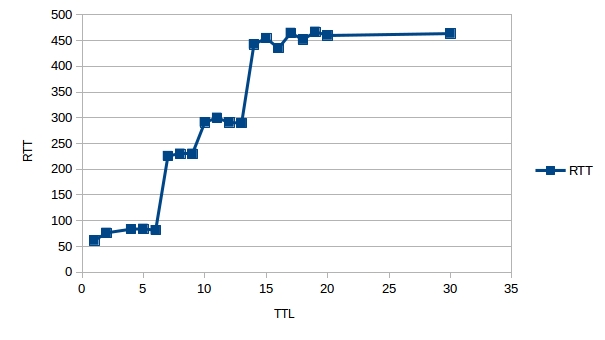
\includegraphics[width=0.7\textwidth]{imagenes/CHI.png}
\end{figure}

\FloatBarrier

En el gráfico, se observan dos grandes saltos en los intervalos 6 a 7 y entre los intervalos 13 a 14. También se destaca otro salto, aunque de menor escala que los anteriores, en el intervalo de 9 a 10. Todos estos saltos parecerían candidatos a ser enlaces intercontinentales.
También se nota un gran intervalo sin respuestas entre los saltos desde el 20 al 30. Posiblemente por ser routers que tienen deshabilitadas las respuestas ICMP.
Por último, se  pueden observar cuatro conjuntos de enlaces con valores de RTT similares.
\\
Vemos a continuación los resultados obtenidos por nuestra herramienta.

\begin{center}
    \begin{tabular}{| l | l | l | l | l | }
    \hline
    Saltos & IP                       & RTT     & DRTT   & País          \\ \hline
    1   	   & 192.168.1.1        & 61.44   & -           & Local         \\ \hline
    2   	   & 201.254.128.1    & 76.47   & 15.02   & Argentina   \\ \hline
    3   	   & *****                    &             &             &                    \\ \hline
    4   	   & 200.51.208.90    & 83.59   & 7.19     & Argentina    \\ \hline
    5   	   & 200.51.240.181  & 84.23   & 0.65     & Argentina    \\ \hline
    6   	   & 213.140.39.118  & 81.47   & -2.77    & Argentina    \\ \hline
    7   	   & 176.52.255.27    & 225.63 & 144.17 & United States \\ \hline
    8   	   & 213.140.37.13    & 230.13 & 4.5       & United States \\ \hline
    9   	   & 63.243.152.141  & 229.97 & -0.17    & United States  \\ \hline
    10   	   & 63.243.152.62    & 291.2   & 61.23   & United States  \\ \hline
    11   	   & 66.110.72.6        & 299.93 & 8.73     & United States  \\ \hline
    12   	   & 66.110.57.82      & 290.7   & -9.23    & United States  \\ \hline
    13   	   & 66.110.59.182    & 289.73 & -0.97    & United States  \\ \hline
    14   	   & 101.4.117.213    & 442.4   & 152.67 & China               \\ \hline
    15   	   & 101.4.117.97      & 454.57 & 12.17   & China               \\ \hline
    16   	   & 101.4.112.105    & 435.1   & -19.47  & China               \\ \hline
    17   	   & 101.4.112.70      & 464.63 & 29.53   & China               \\ \hline
    18   	   & 101.4.116.117    & 451.69 & -12.94  & China               \\ \hline
    19   	   & 101.4.117.29      & 466.94 & 15.25   & China               \\ \hline
    20   	   & 101.4.115.173    & 459.77 & -7.17    & China               \\ \hline
    21  	   & *****                    &             &             &                    \\ \hline
    22   	   & *****                    &             &             &                    \\ \hline
    23   	   & *****                    &             &             &                    \\ \hline
    24   	   & *****                    &             &             &                    \\ \hline
    25   	   & *****                    &             &             &                    \\ \hline
    26   	   & *****                    &             &             &                    \\ \hline
    27   	   & *****                    &             &             &                    \\ \hline
    28   	   & *****                    &             &             &                    \\ \hline
    29   	   & *****                    &             &             &                    \\ \hline
    30   	   & 202.120.127.220 & 463.43 & 3.67    & China          \\ \hline
 \end{tabular}
\end{center}

Nuevamente podemos observar algunos saltos en los que no se obtuvo \emph{ICMP Echo Reply}. La mayoría de los routers que no respondieron, corresponden a equipos ubicados en China. Posiblemente esto se deba a la anomalía de \texttt{traceroute} llamada \emph{Missing Hops}.
\\
Vemos también que los grupos de enlaces con valores de RTT similares que pudimos observar anteriormente en el gráfico, coinciden con el país en el que se encuentran.
\\
Se vuelve a dar el caso del experimento anterior en el que se calcularon valores de dRTT negativos. Como explicamos anteriormente, este podría ser el caso de la anomalía conocida como \emph{False Round-Trip Times}.    
\\\\
Ahora intentaremos inferir cuáles saltos son enlaces intercontinentales mediante la técnica de estimación de John M. Cimbala.
El resultado obtenido por nuestra herramienta fue que los siguientes saltos corresponden a enlaces intercontinentales.

\begin{center}
    \begin{tabular}{| l | l | l | l | l | }
    \hline
    Desde                & Hasta                  & DRTT    & País Desde     & País Hasta    \\ \hline
   66.110.59.182    &  101.4.117.213    & 152.67  & United States & China              \\ \hline
   213.140.39.118  & 	176.52.255.27    & 144.17 & Argentina       & United States  \\ \hline
   63.243.152.141  &  63.243.152.62     & 61.23   & United States  & United States \\ \hline
  \end{tabular}
\end{center}

Los resultados que arrojó la herramienta, confirman la hipótesis que los dos grandes saltos observados anteriormente corresponden a enlaces Intercontinentales. De Estados Unidos a China que posee el dRTT más grande y de Argentina a Estados Unidos.
El otro salto que observábamos, el test lo calculo como un outlier, pero viendo las ubicaciones de los nodos, esto no sería un enlace intercontinental ya que ambos se encuentran ubicados en Estados Unidos. 
\\\\
A continuación veremos en el mapa las direcciones IP de los diferentes saltos, ubicadas según el análisis realizado.

\FloatBarrier

\begin{figure}[ht!]
  \centering
   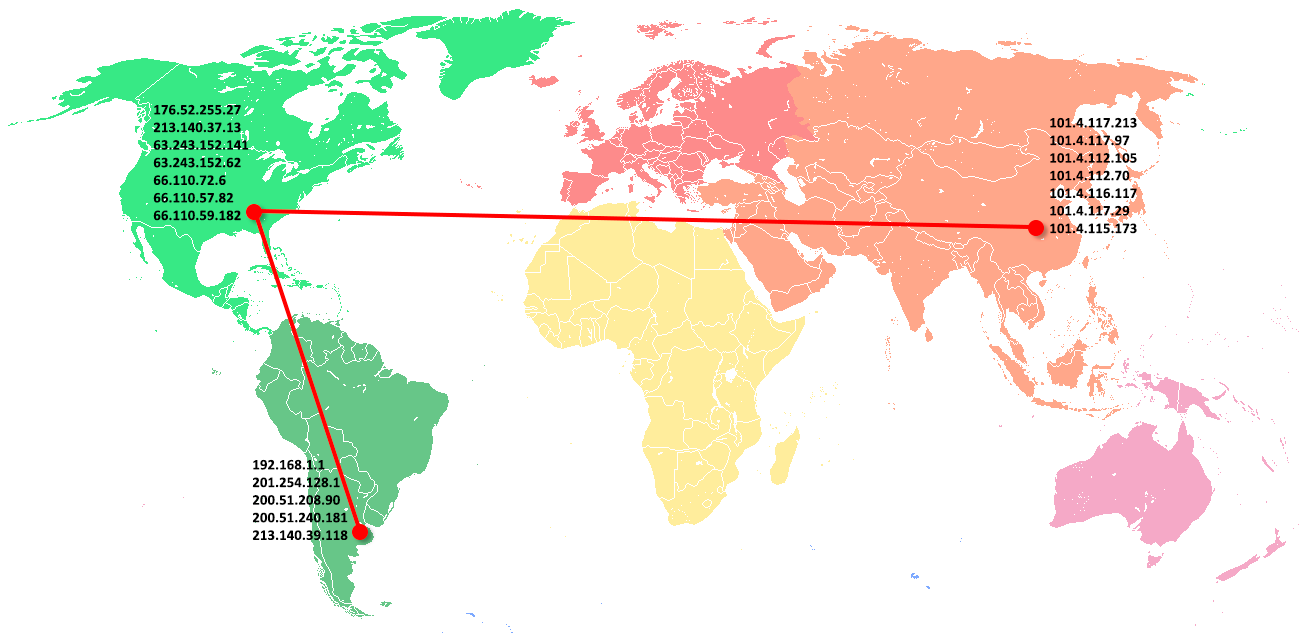
\includegraphics[width=1.0\textwidth]{imagenes/mapaCHI.png}
\end{figure}

\FloatBarrier

\subsection{Universidad de Noruega}
Para el último experimento elegimos una Universidad de un país de Europa.
A continuación analizaremos los datos del experimento de la Universidad de Noruega, de Ciencia y Tecnología (ntnu.edu). 
Veremos el gráfico que muestra los valores de los RTT en cada salto (TTL).

\FloatBarrier

\begin{figure}[ht!]
  \centering
   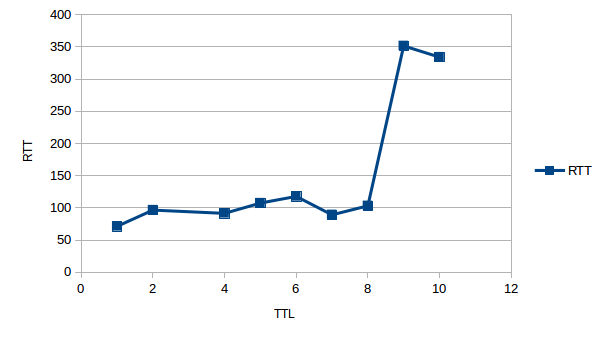
\includegraphics[width=0.7\textwidth]{imagenes/NOR.png}
\end{figure}

\FloatBarrier

En el gráfico, se pueden observar saltos con similar valor de RTT, pero no todos de manera creciente. Esto posiblemente se deba a diferentes tipos de anomalías del \texttt{traceroute}.
También podemos ver que para el último salto el valor del RTT es menor que el del RTT del salto anterior.
\\
Además podemos observar un único gran salto que probablemente pertenezca a un enlace intercontinental.
\\\\
Analizamos los datos obtenidos con nuestra herramienta de traceroute.

\begin{center}
    \begin{tabular}{| l | l | l | l | l | }
    \hline
    Saltos & IP                       & RTT     & DRTT   & País          \\ \hline
    1   	   & 192.168.1.1      & 71.22   & 71.22    & Local         \\ \hline
    2   	   & 201.254.128.1    & 96.5     & 25.28    & Argentina  \\ \hline
    3   	   & *****                    &             &              &                  \\ \hline
    4   	   & 200.51.208.90    & 91.47   & -5.03     & Argentina  \\ \hline
    5   	   & 200.51.240.181  & 107.4   & 15.93    & Argentina \\ \hline
    6   	   & 213.140.39.118  & 117.77 & 10.37    & Argentina \\ \hline
    7   	   & 213.140.35.83    & 89.13   & -28.63   & Argentina \\ \hline
    8   	   & 213.140.53.77    & 103.1   & 13.97    & Argentina \\ \hline
    9   	   & 89.221.43.28      & 351.67 & 248.57  & UK  \\ \hline
    10   	   & 149.3.183.45      & 334.17 & -17.5     & Noruega \\ \hline

 \end{tabular}
\end{center} 

En este caso, se ve solo un salto sin respuesta, posiblemente debido a la anomalía de \texttt{traceroute} \emph{Missing Hops}. También se obtuvieron dos enlaces con dRTT negativo, probablemente por la anomalía \emph{False Round-Trip Times}.
Por último parecería haber un enlace intercontinental en el salto 9, por su alto valor de dRTT comparado con el resto. Además este nodo se encuentra ubicado en UK y el anterior en Argentina.
\\\\
Utilizaremos la la técnica de estimación de John M. Cimbala para verificar si efectivamente el salto 9 en un enlace intercontinental.  
El resultado obtenido por nuestra herramienta fue el siguiente.

\begin{center}
    \begin{tabular}{| l | l | l | l | l | }
    \hline
    Desde                & Hasta                  & DRTT    & País Desde     & País Hasta    \\ \hline
    213.140.53.77   & 89.221.43.28       & 248.57   &   Argentina            &  UK               \\ \hline
  \end{tabular}
\end{center}

Efectivamente lo que intuíamos que era un salto intercontinental fue detectado por nuestra herramienta.
\\\\
A continuación veremos en el mapa las direcciones IP de los diferentes saltos, ubicadas según el análisis realizado.

\FloatBarrier

\begin{figure}[ht!]
  \centering
   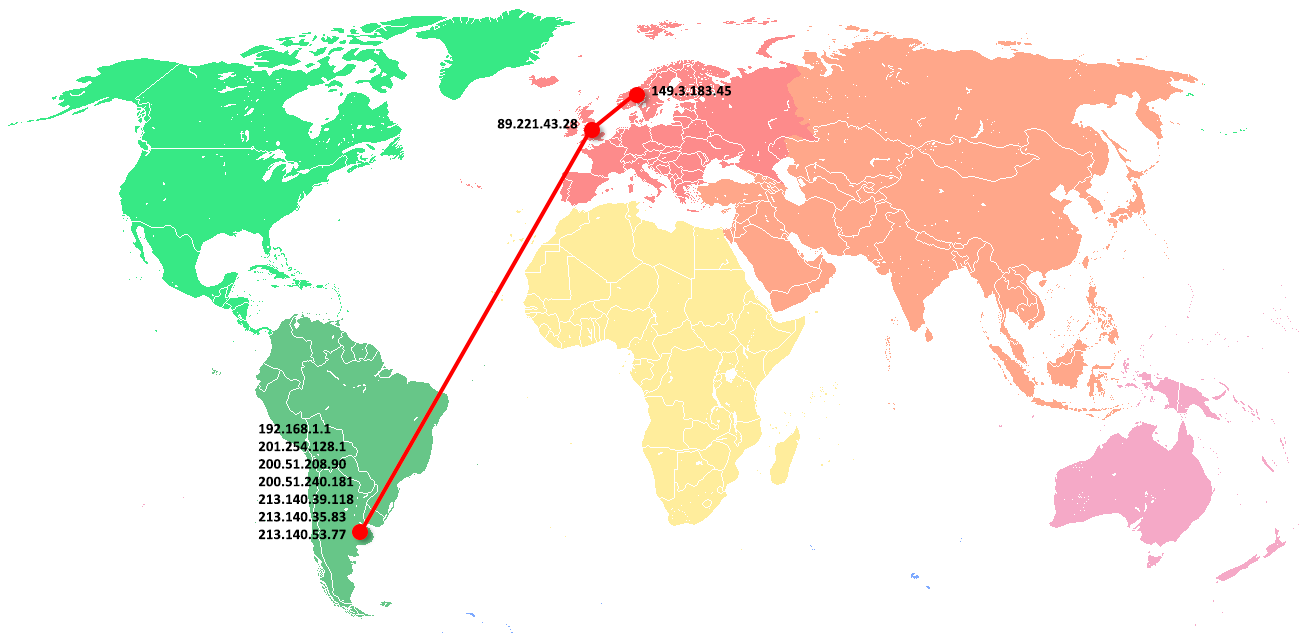
\includegraphics[width=1.0\textwidth]{imagenes/mapaNOR.png}
\end{figure}

\FloatBarrier